\newpage
\section{Specifications}

This section describes the AXI Upsizer IP specifications. This IP uses the AXI 4 Full protocol.

\subsection{Description}

The goal of this IP is to convert data of size X to size Y. The 
interface used is AXI4-MM.

X and Y can take the following values: 32, 64, 128 and 256 bits. 
 
\textbf{Note:} This IP work in one clock domain. 

\begin{figure}[H]
    \centering
    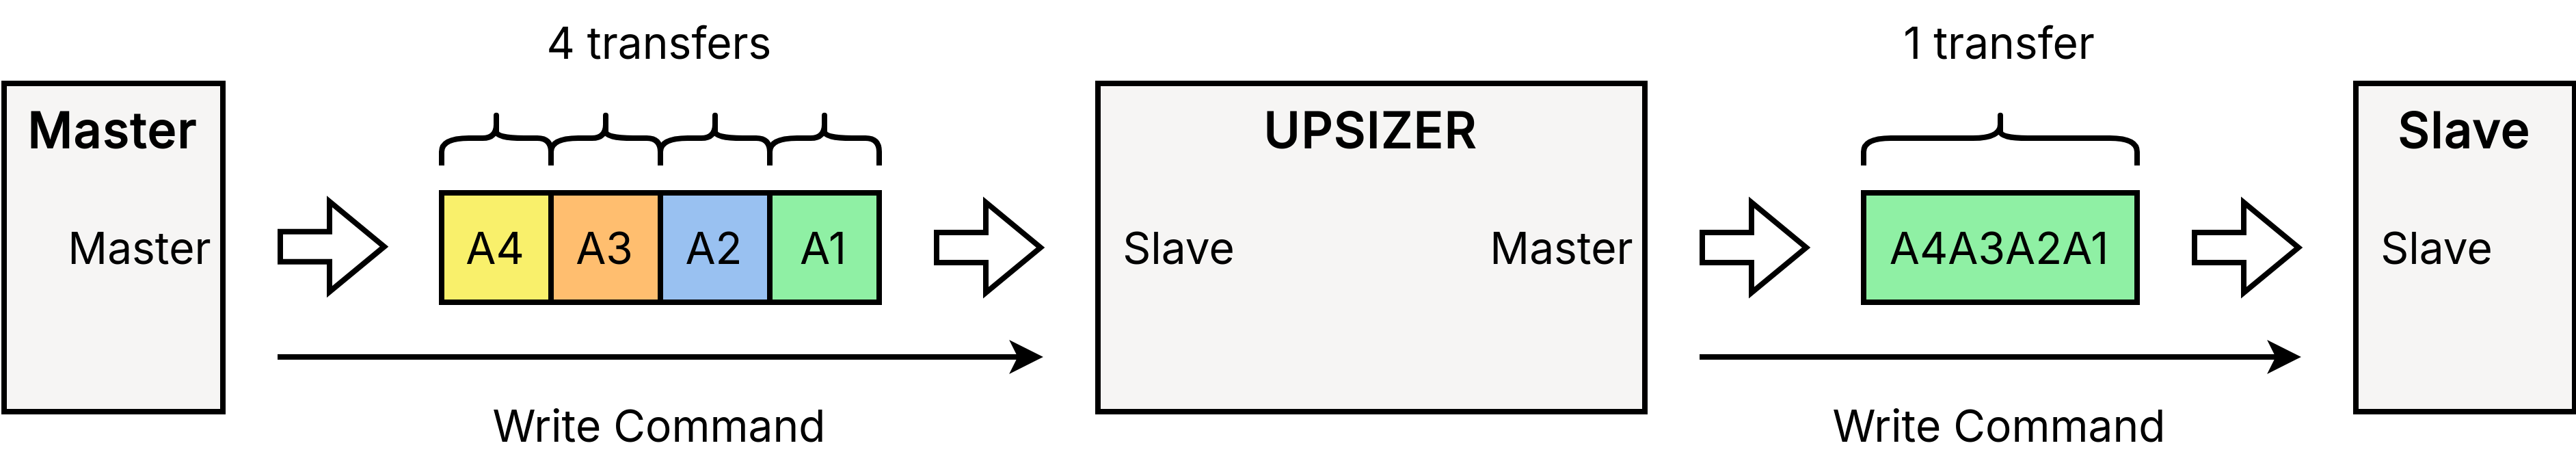
\includegraphics[width=1\linewidth]{images/UPSIZER_PRINCIPLE_WRITE.png}
    \caption{Upsizer Write Principle}
\end{figure}

\begin{figure}[H]
    \centering
    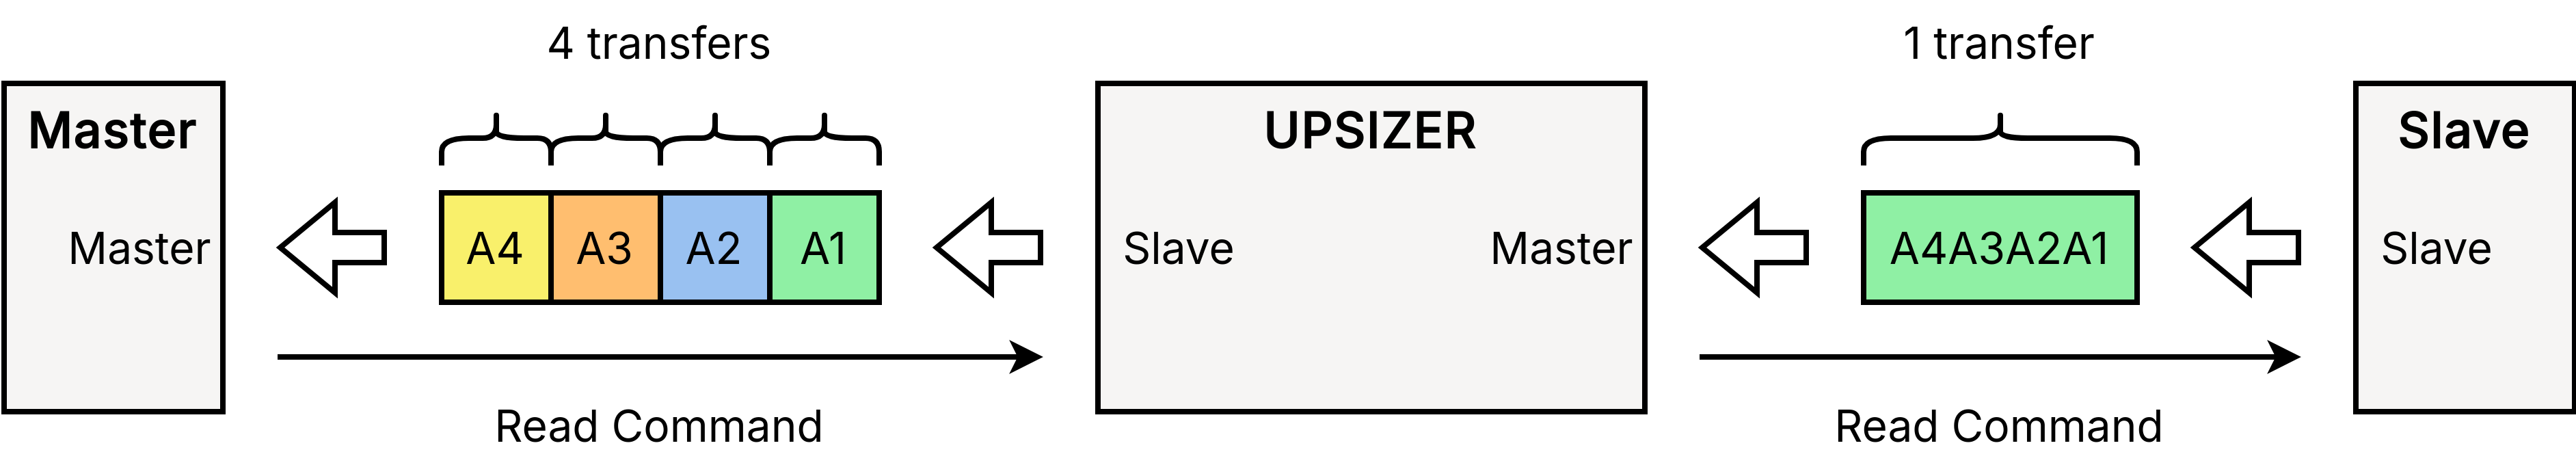
\includegraphics[width=1\linewidth]{images/UPSIZER_PRINCIPLE_READ.png}
    \caption{Upsizer Read Principle}
\end{figure}

\subsection{IP Overview}

\begin{figure}[H]
    \centering
    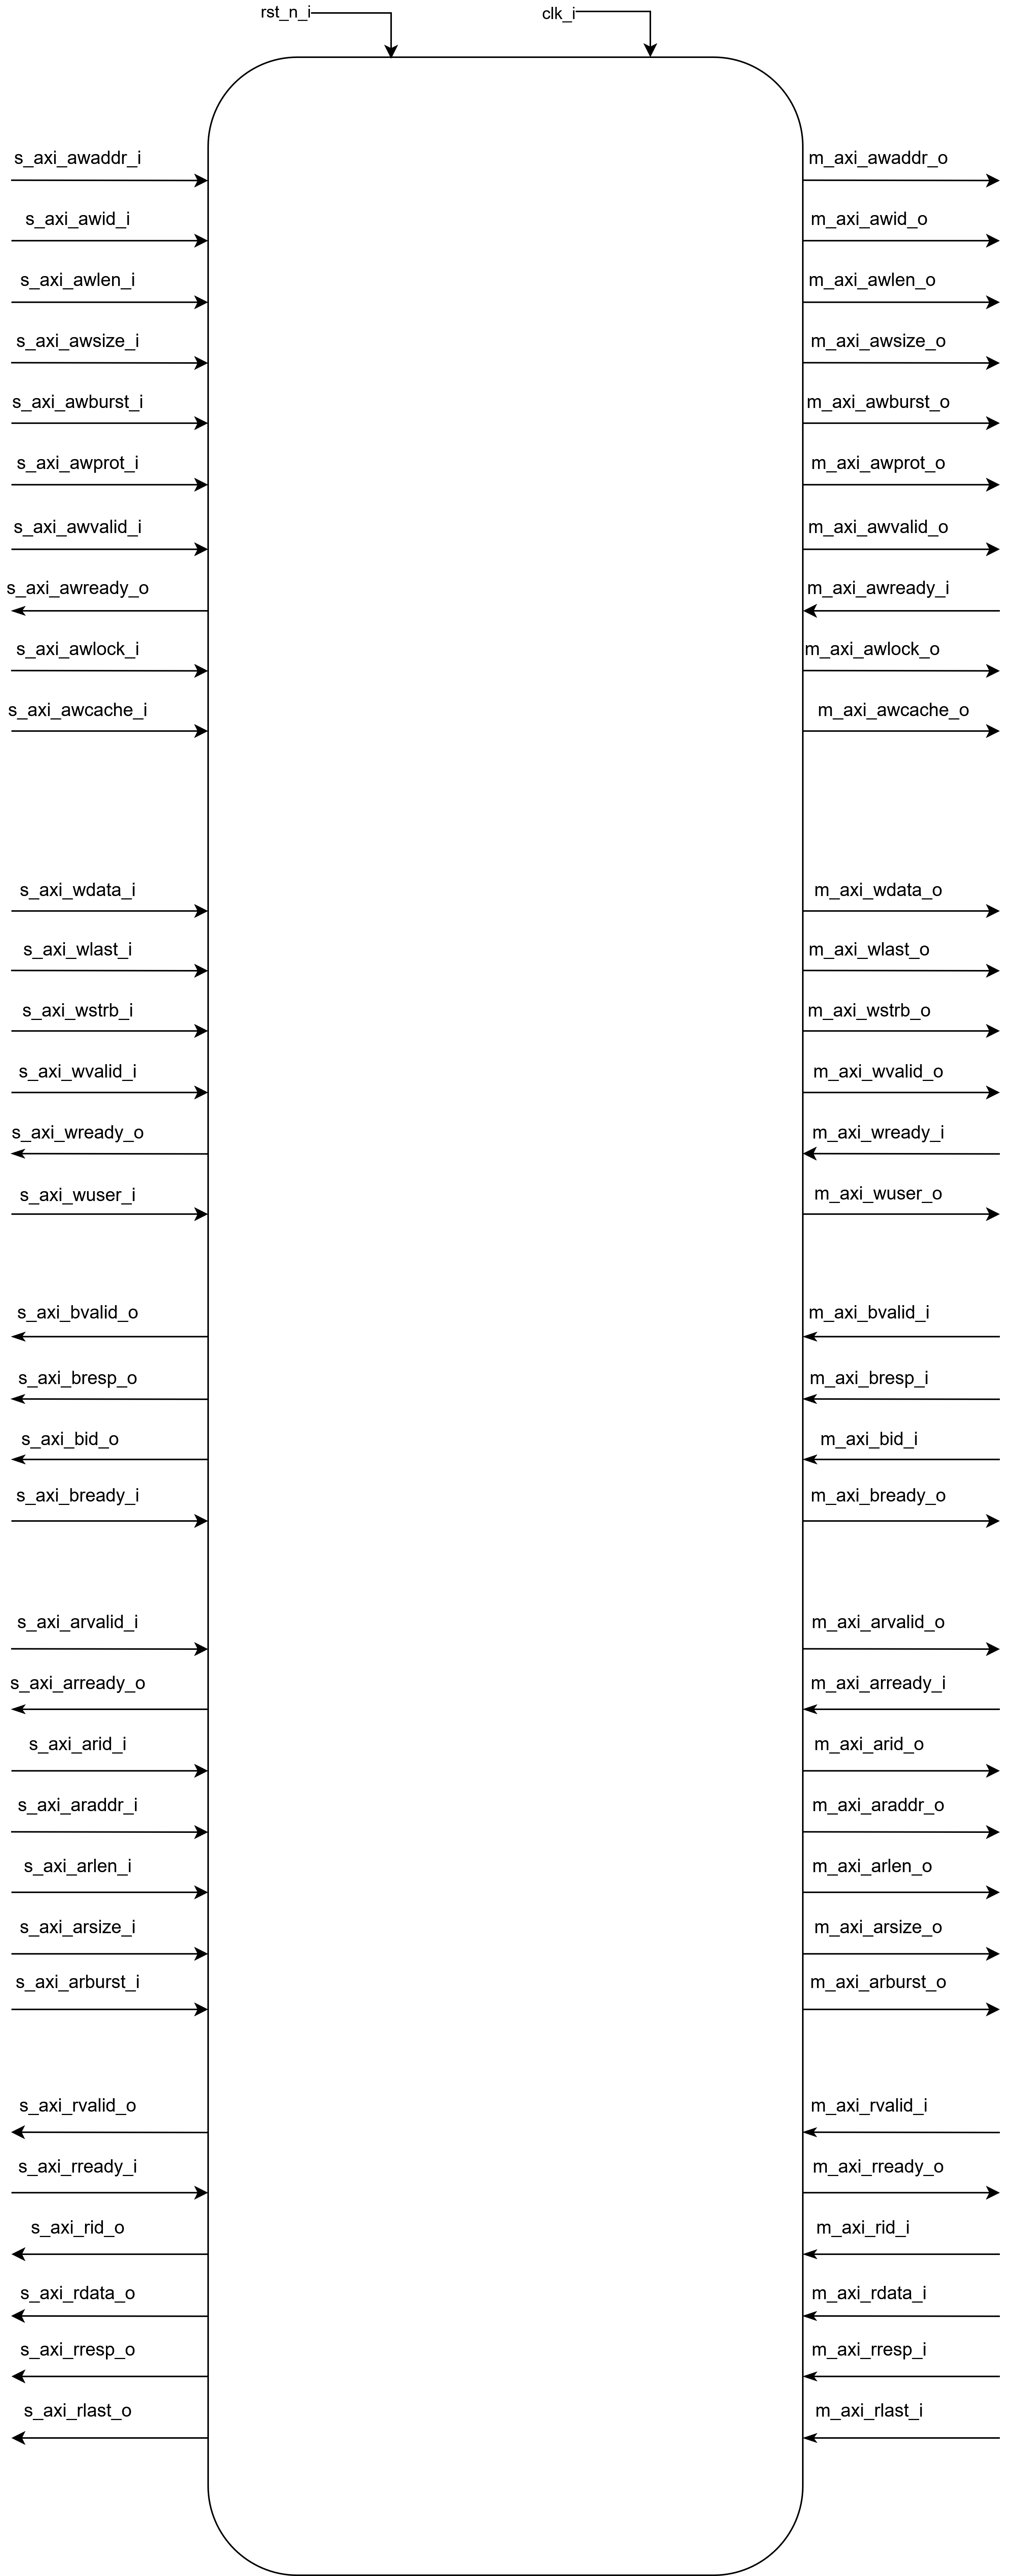
\includegraphics[width=0.55\linewidth]{images/Overview_Upsizer(1).png}
    \caption{IP Overview}
\end{figure}

\subsection{Input \& Output signals}

https://github.com/ZipCPU/wb2axip/blob/master/rtl/demofull.v

Lien d'un fichier expliquant chaque signal si tu veux comparer + c'est déjà en anglais mais a toi de voir

\begin{table}[H]
\begin{threeparttable}
\caption{Global signals}
% \label{keyboard_table}
\begin{tabularx}{\textwidth}{wl{3cm} | wm{3cm} | X}
\hline
\textbf{Name}   & \textbf{Size} & \textbf{Description}                              \\
\hline
clk\_i          & 1 bit         & Global clock signal.                              \\
rst\_n\_i       & 1 bit         & Global reset signal. This signal is active LOW.   \\
\hline
\end{tabularx}
\end{threeparttable}
\end{table}
\begin{table}[H]
\begin{threeparttable}
\caption{Write Request Channel}
% \label{keyboard_table}
\begin{tabularx}{\textwidth}{wl{3cm} | wm{3cm} | X}
\hline
\textbf{Name}   & \textbf{Size} & \textbf{Description}                              \\
\hline
s\_axi\_awaddr\_i          & choice        & Address of first transfer in a transaction.                              \\
s\_axi\_awid\_i            & choice        & Transaction identifier for the write channels.   \\
s\_axi\_awburst\_i         & 2 bits        & Burst type. The burst type determines how the address for each transfer within the burst is calculated. See \underline{\ref{Addresses}} for more details.
\\
s\_axi\_awlen\_i           & 8 bits        & Burst length. The burst length gives the exact number of transfers in a burst. 
 \\
s\_axi\_awsize\_i          & 3 bits        & Burst size. This signal indicates the size of each transfer in the burst.      \\
s\_axi\_awprot\_i           & 3 bits        & The Access attributes for a request which can be used to protect memory against unexpected transactions. \\
s\_axi\_awvalid\_i           & 1 bit        & Write request valid indicator. \\
s\_axi\_awready\_o           & 1 bit        & Write request ready indicator \\
s\_axi\_awlock\_i           & 1 bit        & Asserted high to indicate that an exclusive access is required. \\
s\_axi\_awcache\_i           & 4 bits        & The memory attributes of a request control how a transaction progresses through the system and how caches and buffers handle the request.
bits : \newline
• [0] Bufferable\newline
 • [1] Modifiable\newline • [2] Other Allocate \newline• [3] Allocate
 \\
\hline
\end{tabularx}
\end{threeparttable}
\end{table}


Marking transactions with different IDs allows transactions with different IDs to complete out of order. This means that transactions to faster memory regions can complete without waiting for earlier transactions to slower memory regions.

\begin{table}[H]
\begin{threeparttable}
\caption{Write Data Channel}
% \label{keyboard_table}
\begin{tabularx}{\textwidth}{wl{3cm} | wm{3cm} | X}
\hline
\textbf{Name}   & \textbf{Size} & \textbf{Description}                              \\
\hline
s\_axi\_wdata\_i          & DATA\_WIDTH\slash8        & write data.                              \\
s\_axi\_wlast\_i            & 1 bit        & Indicates the last write data transfer of a transaction   \\
s\_axi\_wstrb\_i         & $\frac{DATA\_WIDTH}{8}$        & Indicates which byte lanes of WDATA contain valid data in a write transaction.\newline
There is one write strobe for each 8 bits of the write data channel, therefore WSTRB[n] corresponds to WDATA[(8n)+7:(8n)].\newline
1 valid, 0 invalid
calculated.  \\
s\_axi\_wvalid\_i           & 1 bit        & Valid indicator.
 \\
s\_axi\_wready\_o          & 1 bit        & Ready indicator      \\
s\_axi\_wuser\_i         & USER\_DATA\_WIDTH        & User-defined extension to write data
Generally, it is recommended to avoid using User signals

 \\
\hline
\end{tabularx}
\end{threeparttable}
\end{table}


\begin{table}[H]
\begin{threeparttable}
\caption{Write Response Channel}
% \label{keyboard_table}
\begin{tabularx}{\textwidth}{wl{3cm} | wm{3cm} | X}
\hline
\textbf{Name}   & \textbf{Size} & \textbf{Description}                              \\
\hline
s\_axi\_bvalid\_o          & 1 bit       &  Write response valid indicator                              \\
s\_axi\_bresp\_o            & 2bits      & Indicates the result of a transaction that uses the write channels.\newline
0b000 OKAY\newline
0b001 EXOKAY\newline
0b010 SLVERR\newline
0b011 DECERR\newline
0b100 DEFER\newline
0b101 TRANSFAULT\newline
0b110 RESERVED\newline
0b111 UNSUPPORTED 

\TODO{A REFAIRE}
   \\
s\_axi\_bid\_o         & ID\_W\_WIDTH        & Transaction identifier for the write channels \newline
 \\

s\_axi\_bready\_i & 1 bit & Ready Indicator\\
\hline
\end{tabularx}
\end{threeparttable}
\end{table}

\begin{table}[H]
\begin{threeparttable}
\caption{Read Request Channel}
% \label{keyboard_table}
\begin{tabularx}{\textwidth}{wl{3cm} | wm{3cm} | X}
\hline
\textbf{Name}   & \textbf{Size} & \textbf{Description}                              \\
\hline
s\_axi\_arvalid\_i          & 1 bit        & Read request valid indicator                              \\
s\_axi\_arready\_o          & 1 bit        & Read request ready indicator transfer of a transaction   \\
s\_axi\_arid\_i         & ID\_R\_WIDTH        & Transaction identifier used for the ordering of read requests, responses, and data.\\
s\_axi\_araddr\_i           & ADRR\_WIDTH        & Address of first transfer in a transaction.
 \\
s\_axi\_arlen\_i          & 8 bits        & The total number of transfers in a transaction, encoded as: Length = AxLEN + 1      \\
s\_axi\_arsize\_i         & DATA\_WIDTH\slash8         & Indicates the maximum number of bytes in each data transfer within a transaction\\
s\_axi\_arburst\_i         & 2 bits         & How the address increments between transfers in a transaction : \newline
•0= FIXED ( same address for every transfer)\newline
•1=INCR   (address for each transfer is an increment of the address for the previous transfer)\newline
•2=WRAP ( same as INCR burst. However, if this incremented address is ((wrap boundary)+ (Size * Length)), then the address wraps round to the wrap boundary.)\newline
•3=RESERVED
 \\
\hline
\end{tabularx}
\end{threeparttable}
\end{table}


\begin{table}[H]
\begin{threeparttable}
\caption{Read Data Channel}
% \label{keyboard_table}
\begin{tabularx}{\textwidth}{wl{3cm} | wm{3cm} | X}
\hline
\textbf{Name}   & \textbf{Size} & \textbf{Description}                              \\
\hline
s\_axi\_rvalid\_o          & 1 bit        & Read request valid indicator                              \\
s\_axi\_rready\_i          & 1 bit        & Read request ready indicator    \\
s\_axi\_rid\_o         & ID\_R\_WIDTH        & Transaction identifier used for the ordering of read requests, responses, and data.\\
s\_axi\_rdata\_o           & DATA\_WIDTH        & Read Data
 \\
s\_axi\_rresp\_o          &  RRESP\_WIDTH         & Response for transactions on the read channels. Must be valid when RVALID is asserted\newline
0b000 OKAY\newline
0b001 EXOKAY\newline
0b010 SLVERR\newline
0b011 DECERR\newline
0b100 PREFETCHED\newline
0b101 TRANSFAULT\newline
0b110 OKAYDIRTY\newline
0b111 RESERVED
    \\
s\_axi\_rlast\_o         & 1 bit         & Indicates the last read data transfer of a transaction
 \\
\hline
\end{tabularx}
\end{threeparttable}
\end{table}


The same applies to the Master side, with inverted In\slash Out. 